\section*{Q3}
Table~\ref{BLEUtable} and figure~\ref{BLEU} illustrate the BLEU scores achieved by rerankers using a variety of feature combinations.

\begin{figure}
	\centering
	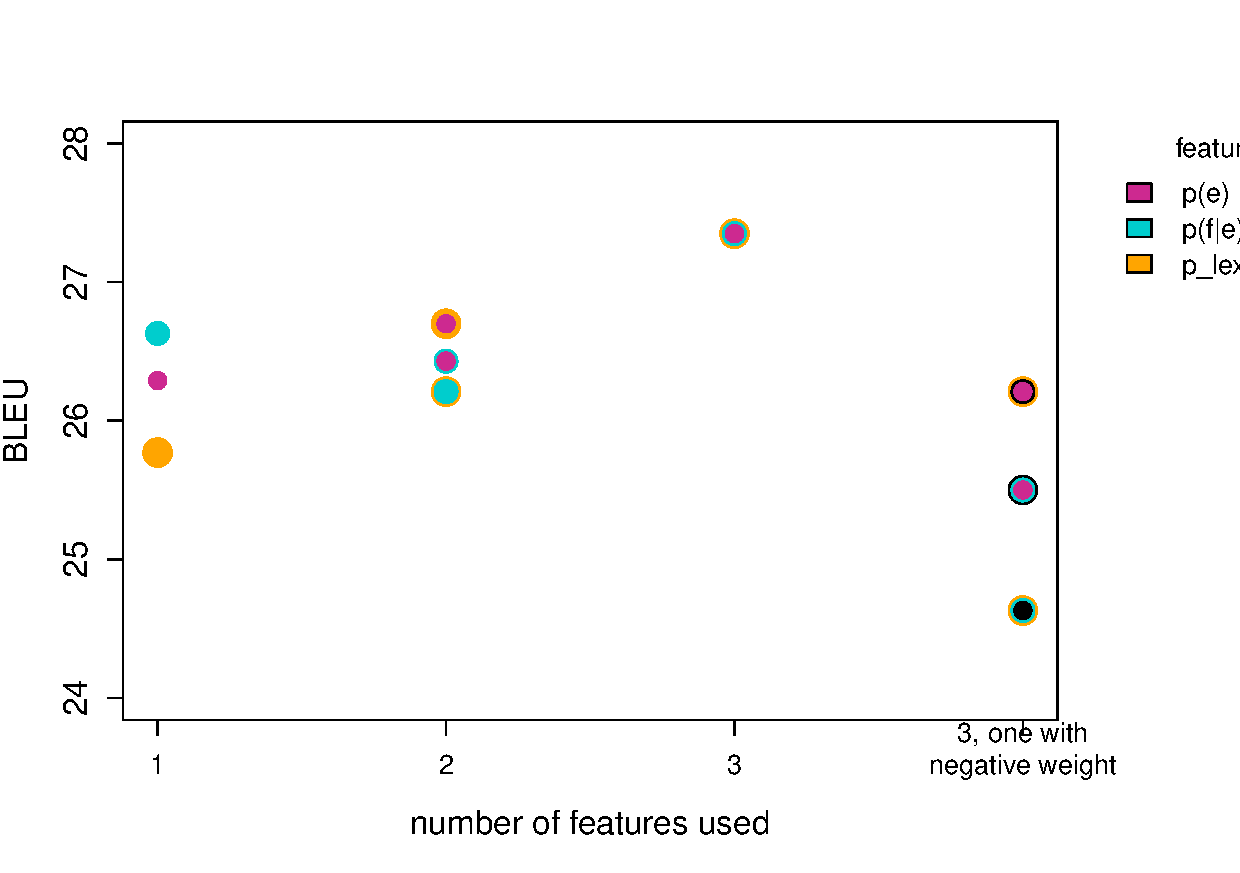
\includegraphics[scale=.65]{figures/q3.pdf}
	\caption{BLEU score as dependent on candidate translation features used for reranking.}\label{BLEU}
\end{figure}

\begin{table}
	\centering
	\begin{tabular}{||c|c|c|c||}
		\hline
		p(e) & p(f|e) & p\_lex(e|f) & BLEU\\
		\hline
		1&1&1&27.35\\
		\hline
		\multicolumn{4}{||c||}{manipulating p(e)}\\
		\hline
		1&0&0&26.29\\
		0&1&1&26.21\\
		-1&1&1&24.63\\
		-1&0&0&24.19\\
		\hline
		\multicolumn{4}{||c||}{manipulating p(f|e)}\\
		\hline
		0&1&0&26.63\\
		1&0&1&26.70\\
		1&-1&1&26.21\\
		0&-1&0&25.58\\
		\hline
		\multicolumn{4}{||c||}{manipulating p\_lex(e|f)}\\
		\hline
		0&0&1&25.77\\
		1&1&0&26.43\\
		1&1&-1&25.50\\
		0&0&-1&24.84\\
		\hline
		\end{tabular}
		\caption{BLUE scores}\label{BLEUtable}
\end{table}

The first thing to note is that the best BLEU score model is achieved when all three features are used, which suggests that all of them contribute useful information. We can approach the question of relative importance of the features from different angles.
\begin{itemize}
	\item Which feature provides the best performance when used alone? : TM likelihood.
	\item Exclusion of which feature causes the largest performance decrease relative to the default system? : LM likelihood
	\item Reversal of which feature causes the largest performance decrease relative to the default system? : LM likelihood
\end{itemize}

The influence of particular features on the BLEU score is quite opaque. There is no single most informative feature. Interestingly, combining TM likelihood with one other feature has a negative influence on the score, but combining it with both brings the score to maximum.  
